\part{Impianti combinati}
\begin{adjustwidth}{2in}{}
	Un ciclo combinato è l'unione delle tecnologie viste fin'ora. 
	
	l'idea di base è che in un gruppo turbogas moderno si riescono a raggiungere temperature massime molto elevate e ciò comporta avere fumi in uscita dall'espansione ancora a temperature elevate (ma a basse pressioni) che possono essere utilizzati, non per la produzione di lavoro, ma per il recupero di calore. 
	
	Si cerca così di valorizzare il contenuto entalpico dei fumi per via termica, convogliando i fumi in un generatore di vapore a recupero che permetta di riscaldare l'acqua di un impianto a vapore. 
	
	In questo modo il ciclo turbogas viene denominato ciclo Topping mentre quello a vapore ciclo Bottoming.  \newline 
	
	Il ciclo combinato presenta molti aspetti positivi
	\begin{itemize}
		\item Rendimento elevato: si immette combustibile soltanto all'interno del ciclo turbogas mentre si produce lavoro sia col turbogas che col vapore
		\item Basso costo: non è necessario un vero e proprio generatore di vapore, mentre la turbina a vapore non raggiunge pressioni elevatissime 
		\item Emissioni contenute: gli unici prodotti della combustione provengono dal ciclo turbogas
	\end{itemize}
\begin{figure}[H]
	\centering
	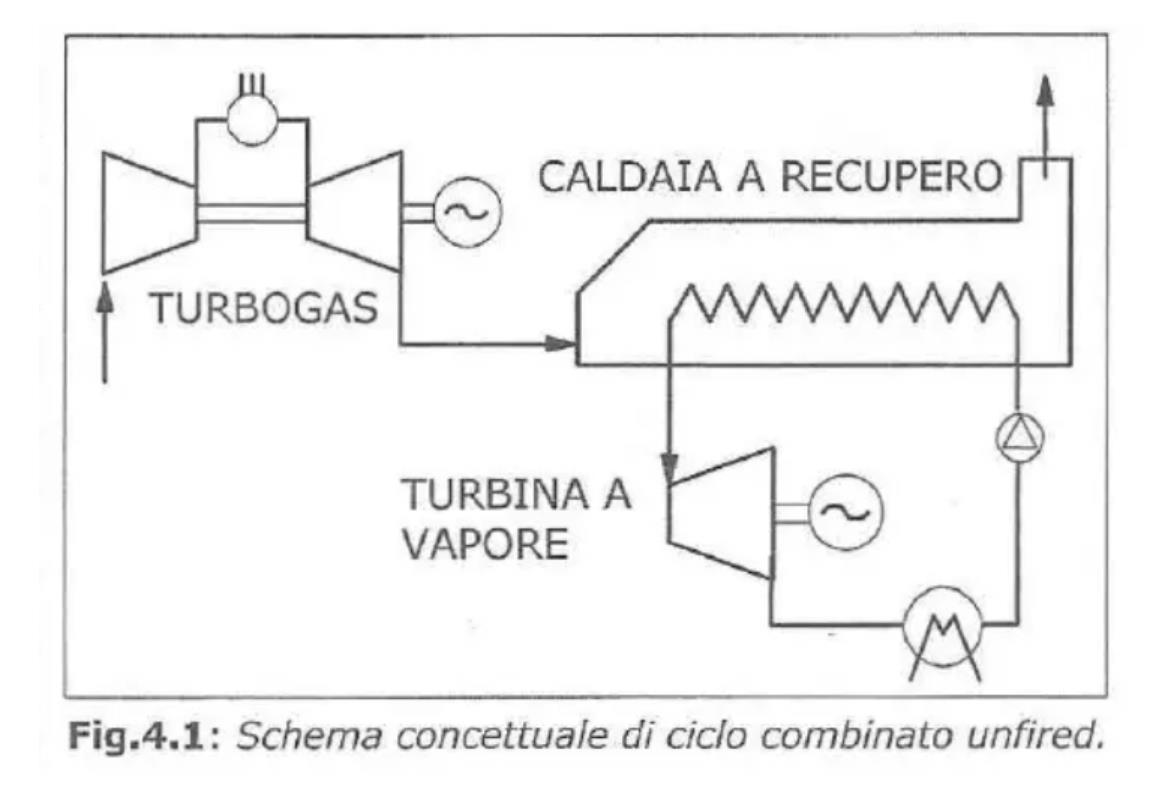
\includegraphics[width=0.5\linewidth]{immagini/impianticombinati}
	\label{fig:impianticombinati}
\end{figure}
	I cicli combinati possono essere 
	\begin{itemize}
		\item \textbf{Mixed}: a ciclo misto, aria viene miscelata a vapore 
		\item \textbf{Unmixed}: se i due fluidi non vengono mai a contatto diretto
		\item \textbf{Unfired}: se non vi è postcombustione dei fumi
		\item \textbf{Fired}: se vie è postcombustione dei fumi.
		
		Questi infatti contenendo una grande quantità di ossigeno, se miscelati con un combustibile possono dar luogo ad una combustione.
		\item \textbf{Green Field}: se vengono sviluppati ex novo con l'intento di costruire da zero un impianto combinato
		\item \textbf{Repowering}: se si adattano impianti preesistenti al ciclo combinato
	\end{itemize}
\end{adjustwidth}




\section{Analisi termodinamica}
\begin{adjustwidth}{2in}{}
	\begin{figure}[H]
		\centering
		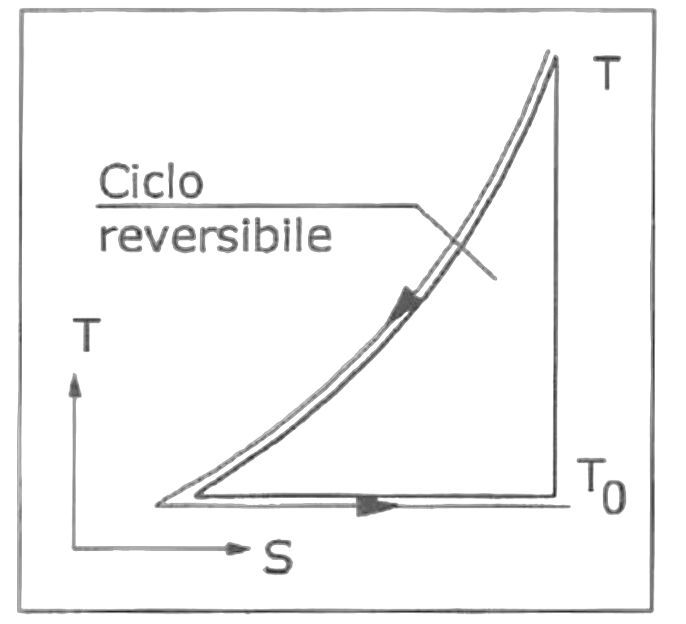
\includegraphics[width=0.5\linewidth]{immagini/impianticombinati1}
		\label{fig:impianticombinati1}
	\end{figure}
	Si sottopone ai gas in raffreddamento un ciclo termodinamico reversibile che massimizza il lavoro estraibile dalla sorgente termica di recupero. \newline 
	
	Si introduce una nuova funzione di stato, l'Energia libera di Gibbs
	\[\Delta G = h-Ts\]
	Questa oltre a individuare se una reazione avverrà spontaneamente o meno, darà indicazioni sulla possibilità di estrarre lavoro, infatti si può scrivere 
	\[\begin{split}
		L_\text{rev} & = \dot{m}[(h-T_0s)-(h_0-T_0s_0)] = \dot{m}(\Delta h - T_0\Delta s) \\ & = \dot{m}\Delta h \left(1-T_0\dfrac{\Delta s}{\Delta h}\right) = Q_{av}\left(1-T_0\dfrac{\Delta s}{\Delta h}\right)
	\end{split}\]
	Dove con $Q_{av}$ si è individuata la potenza termica disponibile, ovvero tutto il calore che sarebbe possibile recuperare raffreddando fino a $T_0$ i fumi. \newline 
	
	Per un gas ideale $c_P=cost$ e allora si può scrivere 
	\[L_\text{rev} = Q_{av}\left(1-\dfrac{T_0}{TML}\right) \qquad \eta_\text{rev} = \left(1-\dfrac{T_0}{TML}\right)\] 
	Dove $TML$ è la temperatura media logaritmica. \newline 
	
	Si definiscono i rendimenti di primo principio e di secondo principio come 
	\[\eta_I = \dfrac{L}{Q_{av}} = \dfrac{L}{Q_1}\dfrac{Q_1}{Q_{av}} = \eta_{th}\chi\]
	Dove $\chi$ è il fattore di recupero del calore.
	\[\eta_{II} = \dfrac{L}{L_\text{rev}} \] 
	In modo che 
	\[\eta_I = \eta_{II}L_\text{rev}\]
	Sebbene non ci si addentri in specifiche definizioni, il concetto principale che deve rimanere è che il ciclo combinato deve massimizzare due effetti per poter essere efficace:$\eta_{th}$ e $\chi$. 
	
	Per il ciclo visto a inizio paragrafo vale tranquillamente $\chi=1$, purtroppo realizzare nella pratica tale ciclo ideale è impossibile perché non esiste fluido che sia in grado di comportarsi allo stesso tempo come un gas nella fase di assorbimento di calore e come un vapore condensate.\newline 
	
	Nell'analisi per individuare il miglior ciclo sottoposto si parte ovviamente da quello di Carnot.
	\begin{figure}[H]
		\centering
		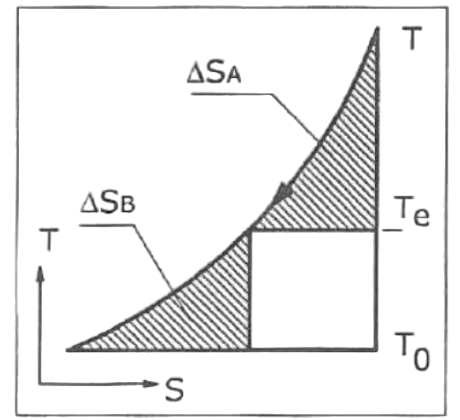
\includegraphics[width=0.5\linewidth]{immagini/impianticombinati3}
		\label{fig:impianticombinati3}
	\end{figure}
	Il calore viene recuperato da $T_0$ a $T_e$ e si individuano due fattori di perdita
	\begin{itemize}
		\item $\Delta S_A$ di cessione causato dallo scambio termico tra gas e fluido ad una determinata $\Delta T$.
		\item $\Delta S_B$ di assorbimento causato dal mancato raffreddamento del gas fino alla $T_0$: tutte le temperature inferiori a $T_e$ non permettono di recuperare il calore.
	\end{itemize}
	Grazie al ciclo di Carnot sottoposto si possono studiare principalmente due casi limite. \newline 
	
	\textbf{Caso limite 1}
	\[
		T_e = T \Rightarrow \begin{cases}
			\eta_{th} = \max\quad\text{Si alza al massimo la temperatura massima} \\
			\xi = 0 \quad\text{non viene recuperato in alcun modo il calore}
		\end{cases}
	\]
	\textbf{Caso limite 2}
	\[
	T_e = T_0 \Rightarrow \begin{cases}
		\eta_{th} = \min \\
		\xi = \max \quad\text{si recupera tutto il calore}
	\end{cases}
	\]
	Tra i casi limite, esiste un valore ottimale?
	
	Dalle definizioni 
	\[\begin{dcases}
		\Delta S_A = c_P\dfrac{T-T_e}{T_e} - c_P\ln\left(\dfrac{T}{T_e}\right) \\
		\Delta S_B = c_P\dfrac{T_e-T_0}{T_0} - c_P\ln\left(\dfrac{T_e}{T_0}\right)
	\end{dcases}\]
	Per massimizzare il rendimento si impone che la somma di questi due elementi sia la minima
	\[\Sigma = \Delta S_A + \Delta S_B = c_P\left[\dfrac{T}{T_e} - 1 + \dfrac{T_e}{T_0} - 1 - \ln\left(\dfrac{T}{T_e}\dfrac{T_e}{T_0}\right)\right]\]
	Volendo ottimizzare il $T_e$ si impone 
	\[\dfrac{d\Sigma}{dT_e} = 0 \Leftrightarrow T_e = \sqrt{TT_0}\]
	Ed il fattore di recupero diventa così esprimibile come 
	\[\chi = \dfrac{T-T_e}{T-T_0}\]
	Ora che si conosce un valore ottimale di temperatura massima raggiungibile dal ciclo sottoposto, quali alternative si possono vagliare rispetto al ciclo di Carnot? 
	\begin{itemize}
		\item \textbf{Passaggi di fase a più livelli di pressione}
		\begin{figure}[H]
			\centering
			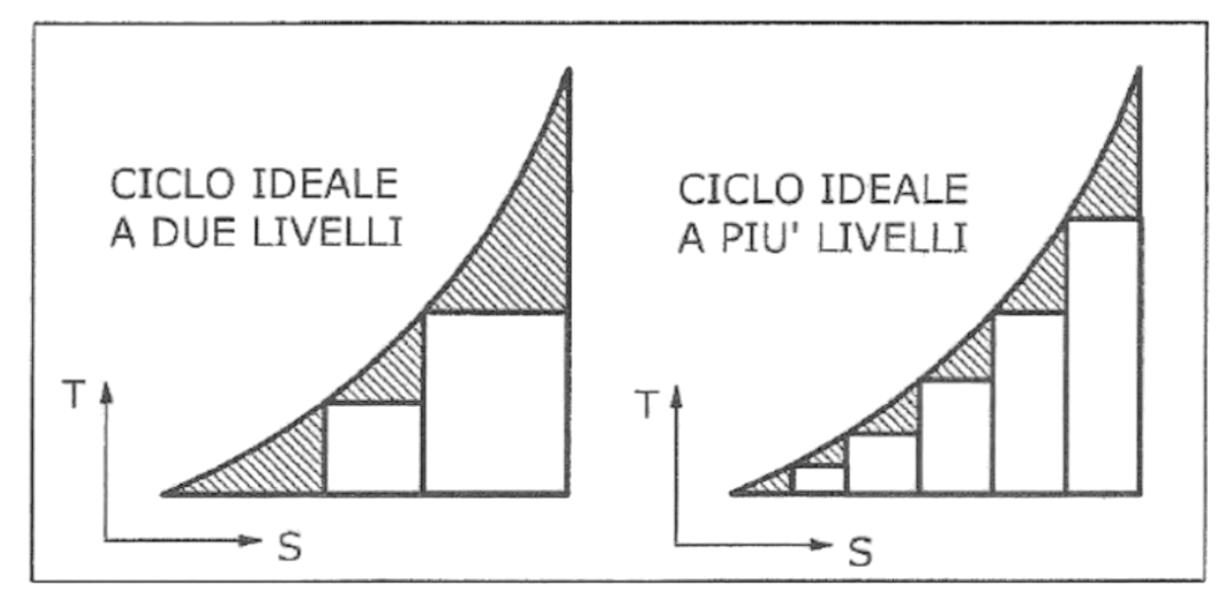
\includegraphics[width=0.5\linewidth]{immagini/impianticombinati4}
			\label{fig:impianticombinati4}
		\end{figure}
		\item \textbf{Impianto a vapore ipercritico}
		\begin{figure}[H]
			\centering
			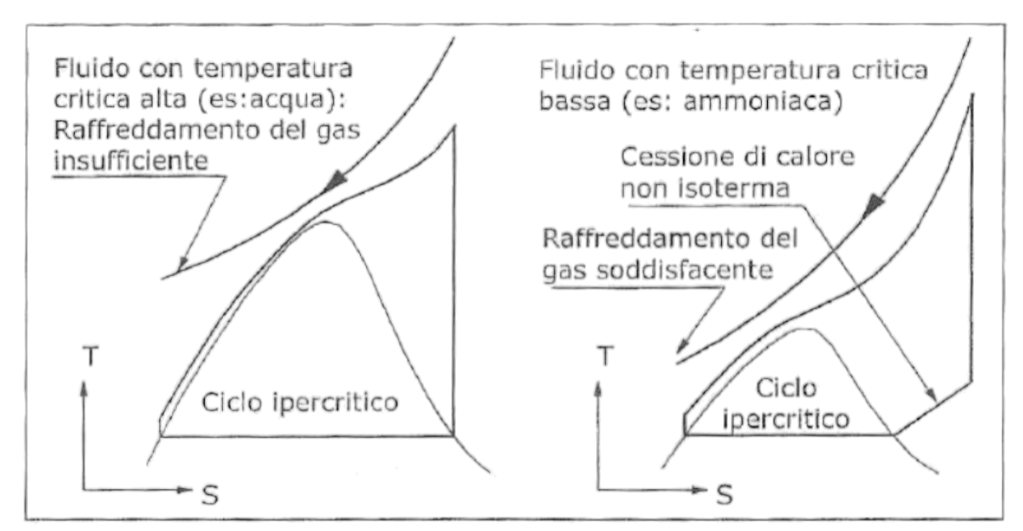
\includegraphics[width=0.5\linewidth]{immagini/impianticombinati5}
			\label{fig:impianticombinati5}
		\end{figure}
		\item \textbf{Compressione interregriferata}
		\begin{figure}[H]
			\centering
			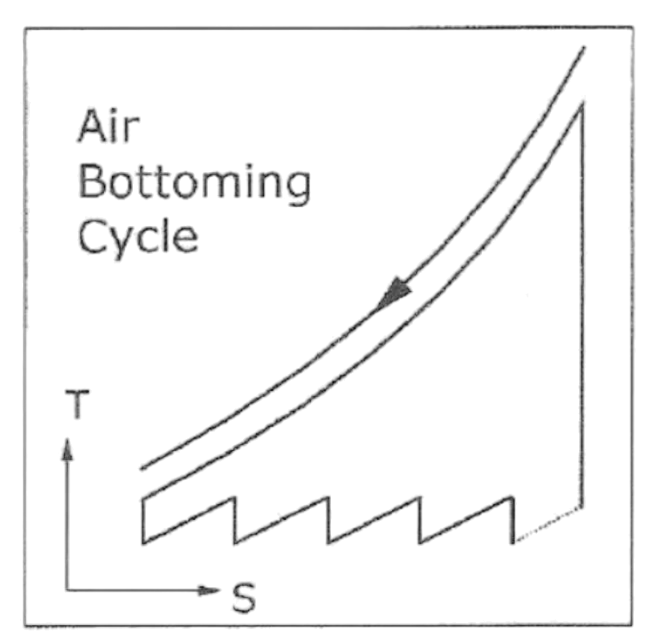
\includegraphics[width=0.3\linewidth]{immagini/impianticombinati6}\
			\label{fig:impianticombinati6}
		\end{figure}
		\newpage
		\item \textbf{Ciclo a vapore con surriscaldamento}
		\begin{figure}[H]
			\centering
			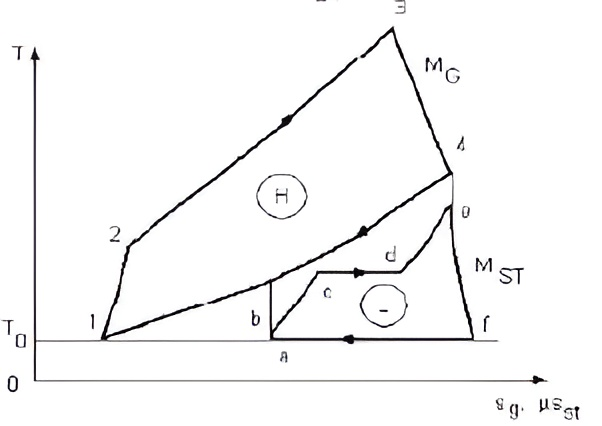
\includegraphics[width=0.5\linewidth]{immagini/impianticombinati7}
			\label{fig:impianticombinati7}
		\end{figure}
		Nonostante la vaporizzazione abbia pendenza costante, tuttavia grazie alla trasformazione all'interno dell'economizzatore e a quella all'interno del surriscaldatore, le due entropie $\Delta S_A$ e $\Delta S_B$ risultano opportunamente scalate, in questo modo si riesce ad aumentare sia $\chi$ che $\eta$ perché aumentano sia calore che temperatura massima del ciclo. 
		
		l'ideale sarebbe eseguire lo stesso ciclo a più livelli di pressione.
	\end{itemize}
	Il rendimento del ciclo combinato sarà 
	\[\eta_{cc} = \eta_{TG} + (1-\eta_{TG}-\chi)\eta_I\approx0.6\]
	È come se si valorizzasse doppiamente il combustibile all'interno del ciclo turbogas. \newline
	
	Ha senso rigenerare?
	
	Il calore del ciclo combinato è già in fase di recupero, così facendo si diminuisce l'effetto di molteplicità delle sorgenti intrinsecamente al ciclo.	
\end{adjustwidth}


\newpage


\section{Generatore di vapore a recupero}
\begin{adjustwidth}{2in}{}
	Il generatore di vapore a recupero si compone delle spesse parti del generatore di vapore classico, cioè economizzatore, surriscaldatore e vaporizzatore, ma questa volta sono posti tutti controcorrente perché non esiste più il problema della resistenza del materiale.
\begin{figure}[H]
	\centering
	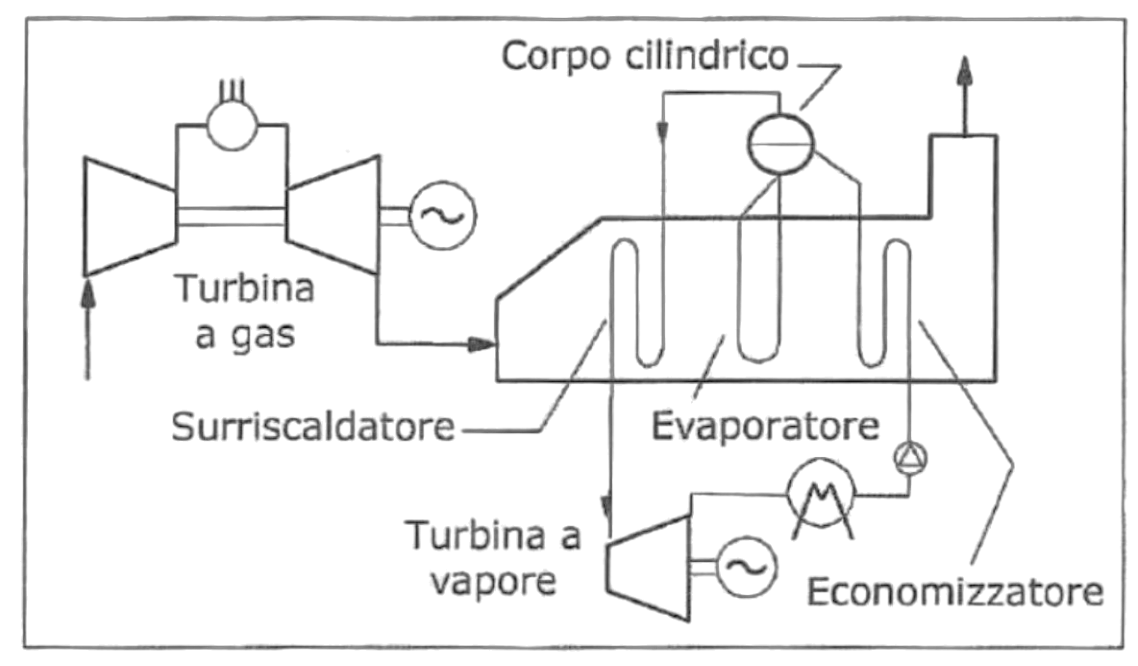
\includegraphics[width=0.5\linewidth]{immagini/impianticombinati8}
	\label{fig:impianticombinati8}
\end{figure}
	All'interno del generatore di vapore a recupero, per acqua e fumi si possono individuare i seguenti andamenti	
\begin{figure}[H]
	\centering
	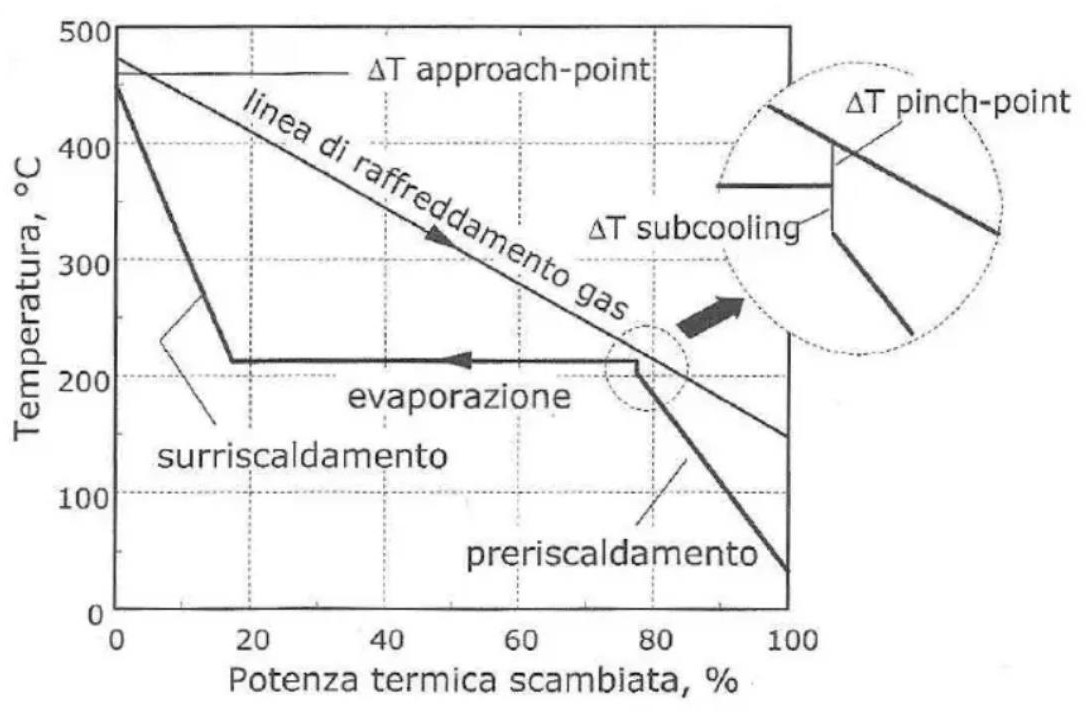
\includegraphics[width=0.7\linewidth]{immagini/impianticombinati9}
	\label{fig:impianticombinati9}
\end{figure}
	Il $\Delta T$ di subcooling (sottoraffreddamento) è necessario perché essendo il liquido più voluminoso del vapore, il passaggio di fase comporterebbe una sostanziale interferenza col regime di moto nei tubi, in questo modo si eliminano i rischi di evaporazione prematura nei fasci tubieri dell'economizzatore. 
\end{adjustwidth}



\subsection{GVR a più livelli di pressione}
\begin{adjustwidth}{2in}{}
	\begin{figure}[H]
		\centering
		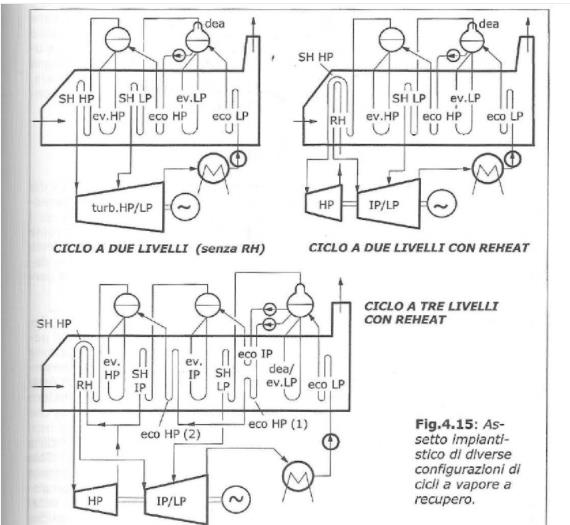
\includegraphics[width=0.8\linewidth]{immagini/impianticombinati10}
		\label{fig:impianticombinati10}
	\end{figure}
	L'obiettivo è quello di minimizzare la temperatura tra gas e liquido che si sta surriscaldando. \newline 
	
	In parallelo ai banchi del surriscaldatore di alta pressione può essere inserito un risurriscaldatore: hanno temperature simili e incontrano i gas caldi praticamente nella stessa posizione.
	\begin{figure}[H]
		\centering
		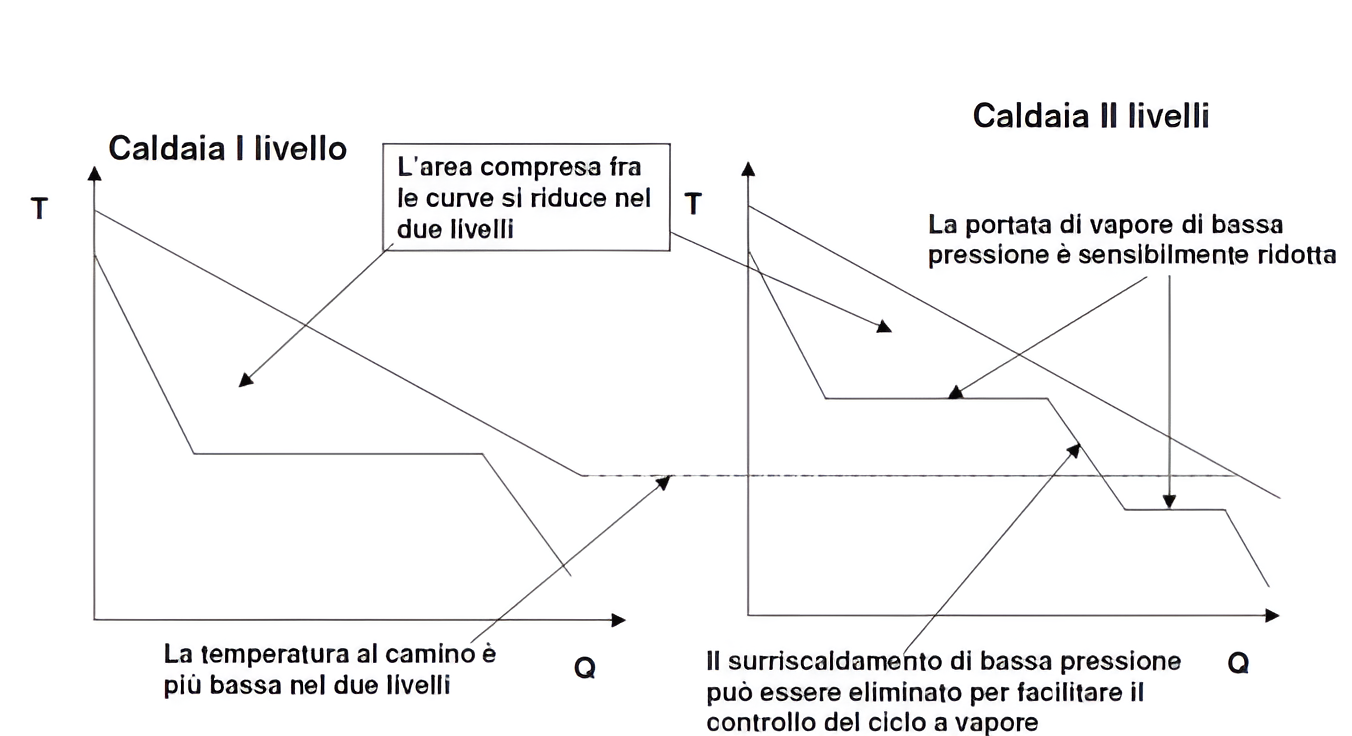
\includegraphics[width=0.8\linewidth]{immagini/impianticombinati11}
		\label{fig:impianticombinati11}
	\end{figure}	
\end{adjustwidth}

\newpage

\section{Variazioni impiantistiche}
\subsection{Ciclo Fired}
\begin{adjustwidth}{2in}{}	
\begin{figure}[H]
	\centering
	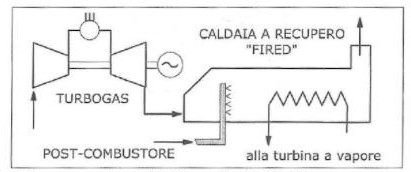
\includegraphics[width=0.5\linewidth]{immagini/impianticombinati12}
	\label{fig:impianticombinati12}
\end{figure}
	Attraverso il ciclo fired si utilizza quel 12$\div$16\% di ossigeno rimasto all'interno dei fumi con l'intento di aumentare la potenzialità della caldaia a recupero ed il fine di produrre più vapore.
	\newline 
	
	Si definisce il rendimento termico
	\[\eta_T = \dfrac{Q_\text{addizionale}}{Q_\text{PostCombustione}}>1\]
	Significa che all'immissione di 1 kWh di combustibile si ottiene più di un 1 kWh di incremento di potenza termica.\newline 
	
	Il ciclo fired interessa notevolmente la pratica impiantistica perché fissata una temperatura di pitch point, entrare nel recuperatore ad una temperatura più alta consente di recuperare più calore ed uscire al camino a minor temperatura.	
\begin{figure}[H]
	\centering
	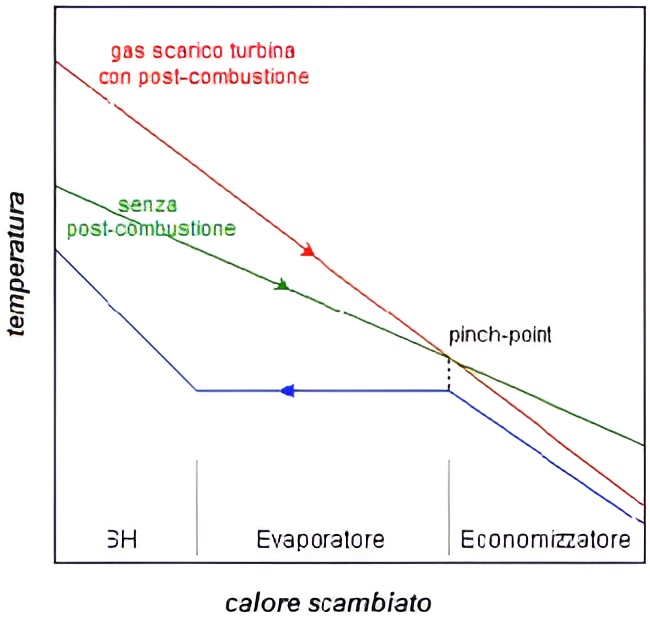
\includegraphics[width=0.5\linewidth]{immagini/impianticombinati13}
	\label{fig:impianticombinati13}
\end{figure}
	Al recupero di maggior calore corrisponde tuttavia una maggiore portata di combustibile, si definisce allora un rapporto sulla quantità di combustibile FPC come il calore del ciclo combinato post combusto diviso il calore del ciclo combinato con la sola combustione al turbogas
	\[FPC = \dfrac{Q_{CC,PC}}{Q_{CC,TG}}\]
	In modo che, il rendimento del ciclo combinato divenga
	\[\eta_{cc} = \dfrac{\eta_{TG} + (1-\eta_{TG}-\chi+FPC)\eta_I}{1+FPC}\]
\end{adjustwidth}

\subsection{Sistemi di Repowering}
\begin{adjustwidth}{2in}{}
	Col sistema di repowering si valorizza una turbina a vapore già preesistente.
	
	Si eliminano generalmente gli spillamenti ad alta pressione e di fa passare il circuito dell'acqua all'interno del GVR. 
	
	Questo sistema tuttavia cambia l'impianto perché ora la turbina - che era stata progettata per un certo numero di spillamenti - vede la sua portata variare: varia la componente $c_m$ dei triangoli di velocità, pertanto sarà necessario verificare se gli spillamenti si possono togliere senza compromettere irrimediabilmente la capacità di compiere lavoro utile della turbina. 
\end{adjustwidth}

\subsection{Sistemi di generazione aggiuntiva di vapore di media pressione}
\begin{adjustwidth}{2in}{}
	all'interno di un impianto a vapore, una pompa, che non è quella di alimento, si occupa di pompare parte dell'acqua proveniente dal degasatore in un circuito secondario all'interno del GVR di un sistema turbogas, col compito di generare vapore a pressione intermedia che verrà intercettato all'uscita dell secondo surriscaldamento, in modo da fornire all'impianto vapore una portata extra evolvente all'interno della turbina di bassa pressione.
\end{adjustwidth}




\subsection{Ricombustione in caldaia}
\begin{adjustwidth}{2in}{}
		I fumi in uscita dal gruppo turbogas vanno a sostituire l'aria in entrata del classico generatore di vapore, in questo modo, immettendo fumi già caldi, si risparmia sul combustibile e si garantisce una portata volumetrica maggiore.
\end{adjustwidth}

\subsection{Trasformazione del ciclo a vapore in un ciclo unfired}
\begin{adjustwidth}{2in}{}
	All'interno di un impianto a vapore si sostituisce il generatore di vapore con un GVR, questo produce più portata di vapore. 
\end{adjustwidth}